\section{Tests}
\subsection{Unit Tests}

\subsection{Hydro Tests}
\subsection{Linear Wave}
Sound waves provide the mechanism to transport disturbances in a fluid. An
elementary test problem is the ability maintain wave propagation of small
disturbances. Given a fluid in equilibrium with constant density $\rho_0$,
pressure $p_0$ and zero velocity $\mathbf{v}=0$ with perturbations of the form
\begin{equation}
	\begin{array}{rcl}
		\rho & = & \rho_0 + \delta\rho(x,t) \\
   		 p & = & p_0 + \delta p(x,t) \\
    	\mathbf{v} & = & \delta\mathbf{v}(x,t),
    \end{array}
\end{equation}
and maintaining terms to first order in the Euler equations produce the wave
equation for each variable with a wave propagation speed equal to the fluid's sound speed 
$c_s$. Thus, setting a small disturbance 
will propagate with a finite velocity maintaining its form.

We set up a 2d box of unit length with constant $\rho_0=1.0$, $p_0=3/5$, $\mathbf{v}=0$,
and $\gamma=5/3$ with periodic boundary conditions. A sinusoidal wave in the x direction of 
the form $\delta\rho(x,t) = Asin(kx + wt)$ with $k=w=2\pi$ and $A=10^{-6}$ is added at time 
$t=0$. The remaining disturbances can be specified through $\delta\rho$ by the following
\begin{equation}
	\begin{array}{rcl}
        \delta \mathbf{v}(x,0) & = & \left(\frac{w}{k}\right)\delta
        	\rho(x,0)/\rho_0\mathbf{\hat{x}}\\
        \delta p(x,0) & = & \left(\frac{w}{k}\right)^2\delta\rho(x,0).
    \end{array}
\end{equation}
The values chosen produce waves traveling rightward with a velocity of 1. The simulation is
ran for 1 time unit such that the waves return to its' initial position at time $t=0$. 
Moreover, we study the convergence behavior by comparing the final state of the density to 
the initial density by computing the $L1$ norm,
\begin{equation}
	L1 = \frac{1}{N^2}\sum_i \left| \rho_i - \rho(x_i) \right|,
\end{equation}
where $\rho_i$ is final density at position $x_i$ and $\rho(x_i)$ is the density at t=0
at position $x_i$ and $N$ is the number of cells per dimension. Five simulations where ran
with varying resolution $N=10, 20, 40, 80, 160$. The initial particles where laid out in a
Cartesian grid and the mesh was allowed to move with the fluid velocity. All simulations
where performed with linear reconstruction and the HLLC solver.
\begin{figure}
    \begin{center}
        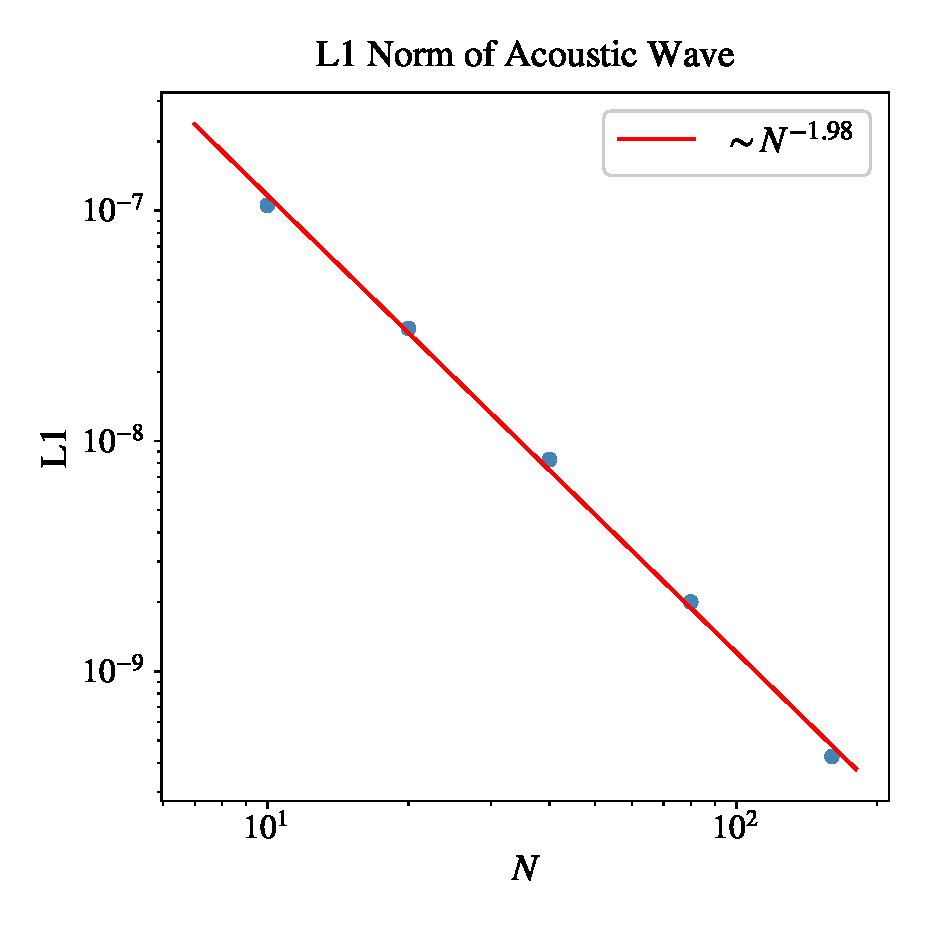
\includegraphics[width=0.4\textwidth]{figures/acoustic-wave-l1.eps}
        \caption{L1 norm of acoustic wave problem in 2d. Blue points are results
        of simulation from different resolutions overlaid by a linear fit showing
        the convergence is approximately second order.}
        \label{fig.acoustic}
    \end{center}
\end{figure}
Figure \ref{fig.acoustic} shows the $L1$ norm as a function of grid cells per dimension.
As expected, the convergence rate is approximately second order in time and space for
this smooth problem. In the presence of shocks or other discontinuities it is not expected
to have such convergence.

\subsubsection{Sod Shock Tube}
To examine the ability of the code to handle shock propagation we perform the Sod problem. The problem
consists of two different constant states at rest separated at the midpoint of the x axis. A discontinuity
exist in the density and pressure at the midpoint. At $t=0$ the high density region flows into the
lower density region. The flow produces a rarefaction, discontinuity, and a shock wave emanating from the
density discontinuity. Thus, this problem creates a great test for the codes ability to capture the tree
wave types.

For our initial setup we use a unit box in 2d with reflective boundary conditions, linear
reconstruction and the HLLC solver. The discontinuity lies along the x axis at 0.5.
The density and pressure are defined as follows
\begin{equation}
	\rho = \left\{
      \begin{array}{@{}ll@{}}
        	1.0 & \text{for}\ x \leq 0 \\
            0.125 & \text{for}\ x > 0
    	\end{array}\right.
\end{equation}
and
\begin{equation}
	p = \left\{
      \begin{array}{@{}ll@{}}
        	1.0 & \text{for}\ x \leq 0 \\
            0.1 & \text{for}\ x > 0
    	\end{array}\right.
\end{equation}
with $\gamma = 1.4$. The particles are laid out in a Cartesian grid and the simulation is evolved
until $t=0.15$. The number of particles per dimension is chosen to be $N=120$.
\begin{figure}
    \begin{center}
        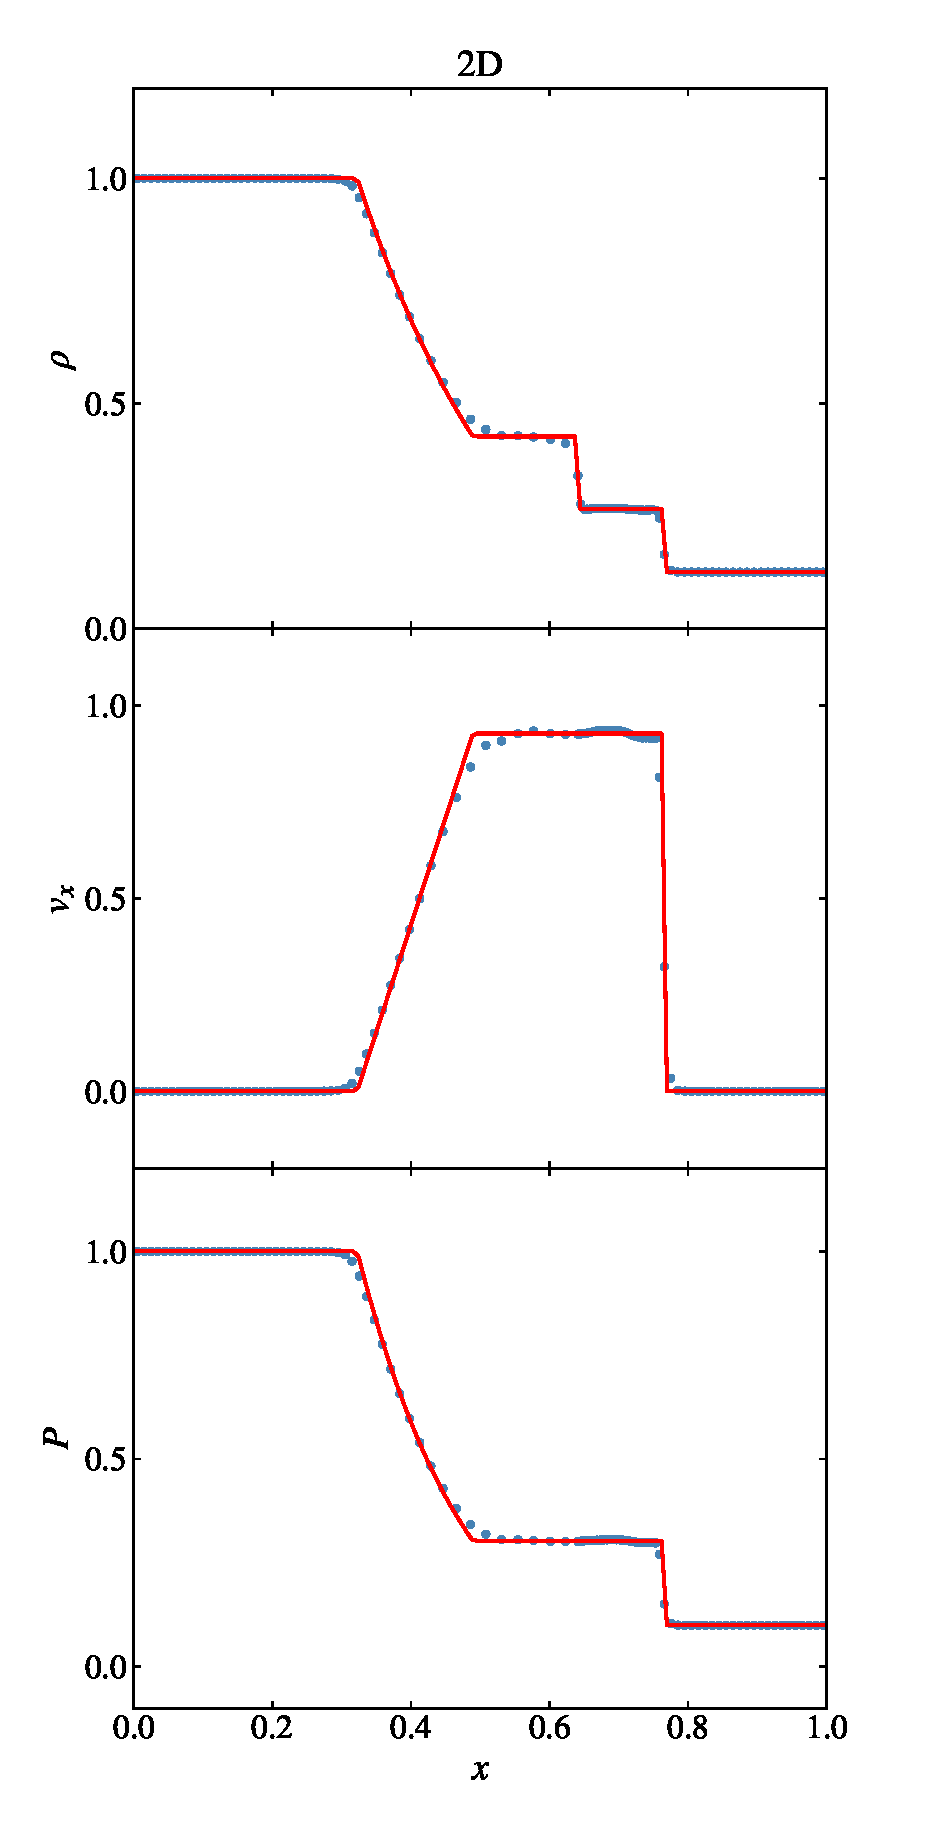
\includegraphics[width=0.4\textwidth]{figures/sod_2d.eps}
        \caption{Profiles of density, velocity and pressure of the Sod simulation. Light blue points are the simulation
        while the red line is the exact solution.}
        \label{fig.sod}
    \end{center}
\end{figure}
Figure \ref{fig.sod} plots all the points of the simulation for density, the x-component of
the velocity and pressure. The red line is the analytical solution. We see the shock is
well resolved as is the contact discontinuity. Further the Lagrangian nature of the code
can be seen as many particles have been squeezed between the contact discontinuity and the
shock front while particles in the rarefaction have been spread out.

\subsection{Explosion}
\begin{figure}
    \begin{center}
        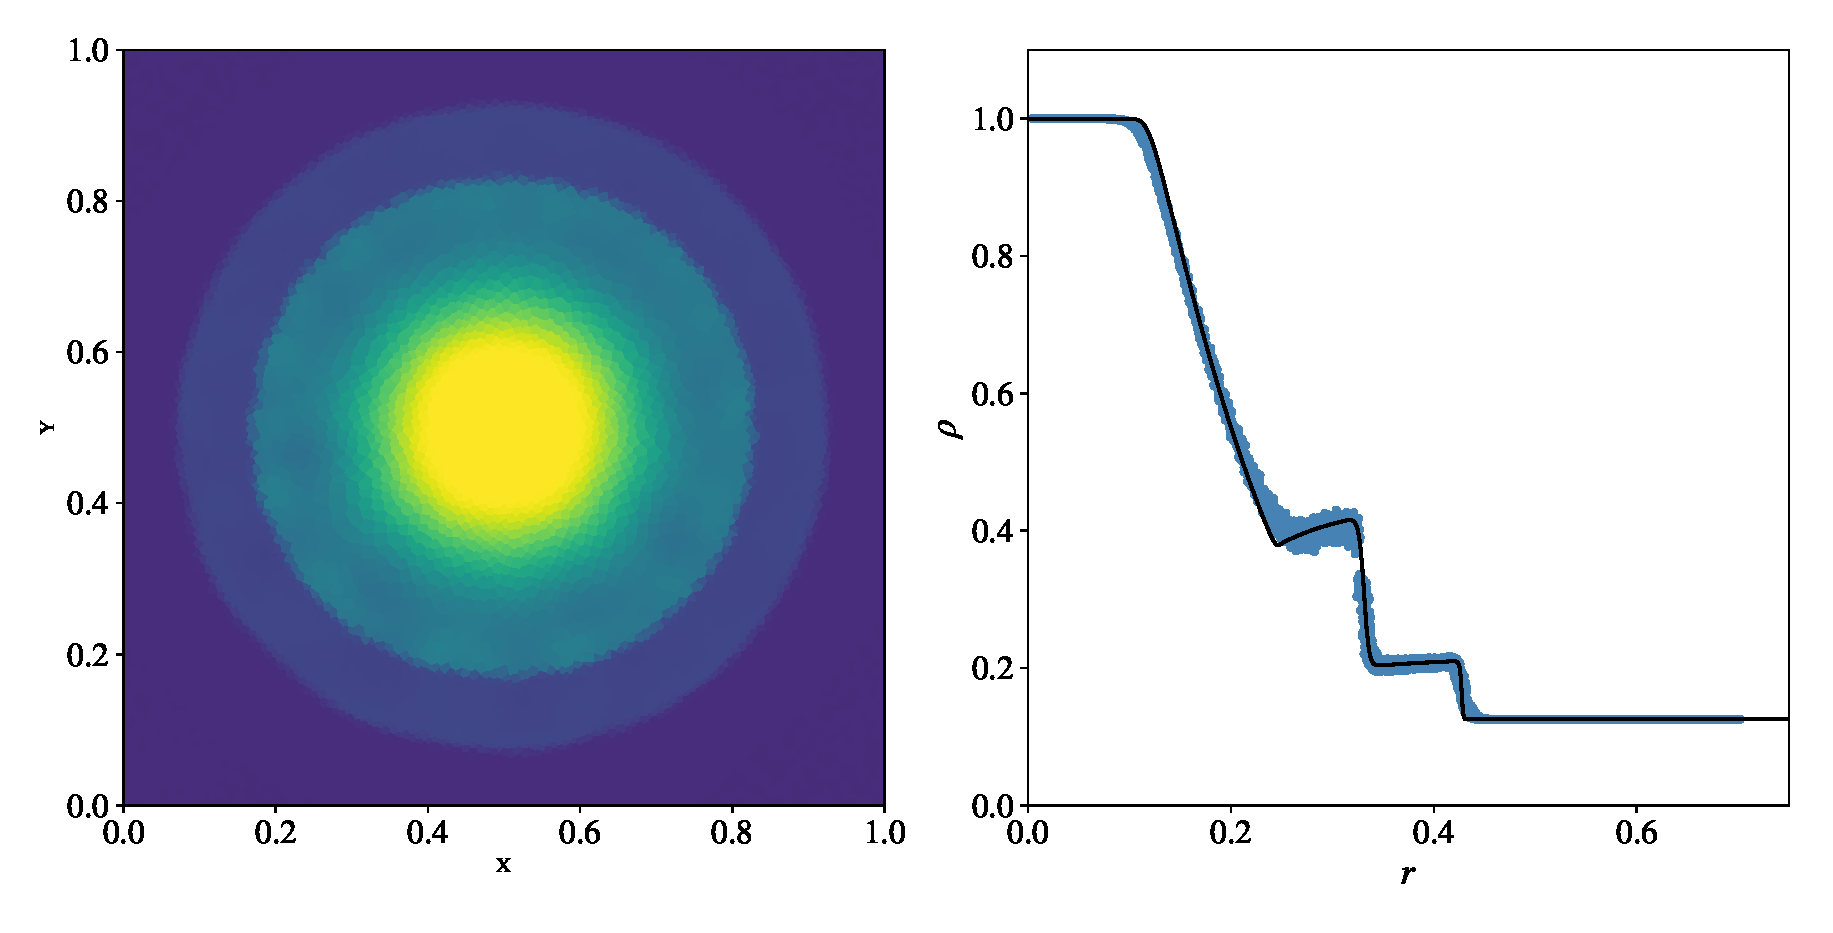
\includegraphics[width=0.9\textwidth]{figures/explosion_2d.eps}
        \caption{Density profile of Sedov-Taylor blast wave problem. Left is the 2D version with an initially
        while the red line is the exact solution.}
        \label{fig.explosion_2d}
    \end{center}
\end{figure}
An analog to the Sod problem is the 2D explosion problem. Like the Sod problem, the domain
is partition into two constant regions. However, the higher density region is now a circular
region of radius $r$ centered in a unit box. Similar to the Sod problem, the initial 
conditions generate a shock, contact discontinuity and rarefaction wave. However, in this case
the waves are now a circular shock wave traveling radially outward, a circular contact
discontinuity traveling in the same direction, and a rarefaction wave traveling towards the
center.

We use the same values as the Sod problem except we restrict the higher density values onto
the center of domain with radius $r=0.25$. Further, instead of using a Cartesian grid we sample
particles uniformly for a unit square and perform 10 iterations of Lloyds algorithm. 

Figure \ref{fig.explosion_2d} shows the density map and density profile. Clearly the cells
density matches the analytical solution in red. Further, the solution captures all three waves
even though the mesh was built in a random fashion. This an important difference over Eulerian
codes, since Lagrangian codes are not constrained to any initial particle placement. Therefore
one can reach better accuracy by placing the particles in way that exploit the problem. We will
see a later example of this in the Evrards problem.

\subsection{Gresho vortex}
Our next problem will test stability of the code. Gresho and Chan cite, introduced an interesting
problem to test for conservation of angular momentum. A vortex in a unit 2D box with constant 
density $\rho=1$ is setup with the following angular velocity
\begin{equation}
	v_\phi (r) = \left\{
      \begin{array}{@{}ll@{}}
        	5r & \text{for}\ 0 \leq r < 0.2 \\
            2-5r & \text{for}\ 0.2 \leq r < 0.4 \\
            0 &\text{for}\ \geq 0.4
    	\end{array}\right.
\end{equation}
The angular velocity of the vortex grows linearly as one moves radially outward from
the center until midway of the disk. Then the velocity decreases linearly until it
vanishes at the rim of the disk. This produces triangular shape velocity profile.
The corresponding pressure is
\begin{equation}
	P\phi (r) = \left\{
      \begin{array}{@{}ll@{}}
        	5 + 25/2r^2 & \text{for}\ 0 \leq r < 0.2 \\
            9+25/2r^2 - 20r + 4\ln(r/0.2) & \text{for}\ 0.2 \leq r < 0.4 \\
            3 + 4\ln(2) &\text{for}\ \geq 0.4.
    	\end{array}\right.
\end{equation}
The pressure is chosen such that the pressure gradients balance the centrifugal forces
generated by the rotation. Thus producing a solution that is independent of time.
\begin{figure}
    \begin{center}
        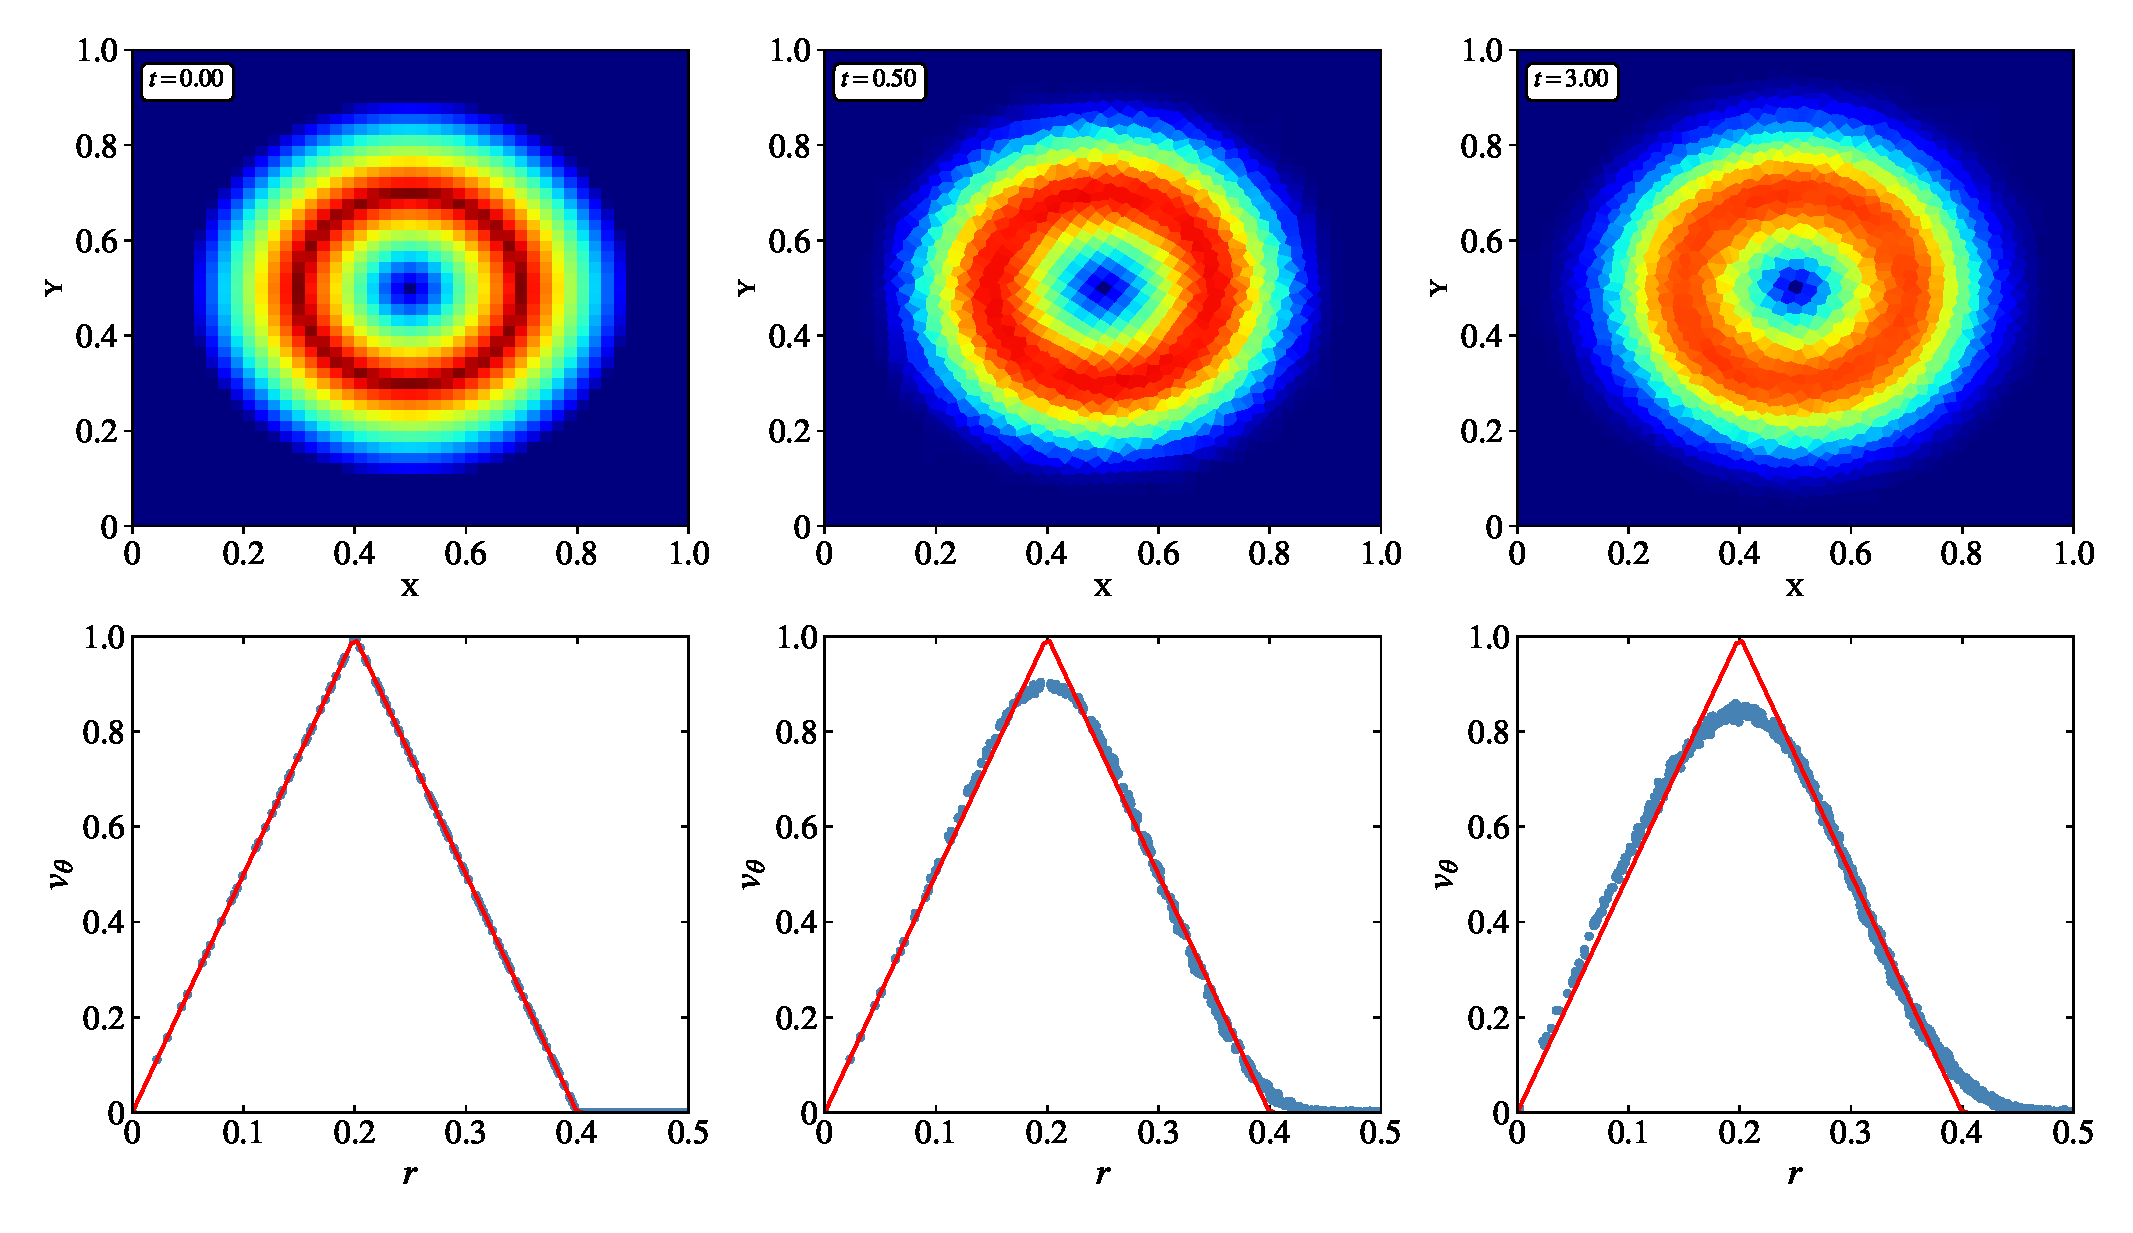
\includegraphics[width=0.9\textwidth]{figures/gresho_vortex.eps}
        \caption{Density profile of Sedov-Taylor blast wave problem. Left is the 2D version with an initially
        Cartesian mesh of $45 \times 45$. Right is the 3D version with an initially Cartesian mesh of 
        $45 \times 45 \times 45$. Light blue points are the density a radius $r$ from the center of the explosion
        while the red line is the exact solution.}
        \label{fig.gresho_vortex}
    \end{center}
\end{figure}



\subsubsection{Sedov-Taylor}
Another test generates a shock is the Sedov-Taylor blast wave problem. In this problem a homogeneous
gas is injected with a large amount of energy in a point-like region at the center of the domain.
A spherical shock is created emanating from the center. The shock propagates radially outward
sweeping mass into a thin shell and creating a cavity behind the shock. The problem has a well known
analytical self-similar solution cite. Applying the Rankine–Hugoniot at the shock front the density
jumps to a maximum compression of
\begin{equation}
	\rho_{\mathrm{max}}/\rho = (\gamma + 1)/(\gamma - 1),
\end{equation}
for $\gamma = 5/3$ this amounts to a max value of 4.

We consider the 2D and 3D case. A unit box is setup with particles in a Cartesian grid of size
$45\times 45$ and $45 \times 45 \times 45$ for 2D and 3D respectively. The stationary gas has
a constant density of $\rho = 1.0$ and pressure $P = 10^{-6}$ with $\gamma=5/3$. The simulation is
allowed to run to time $t=0.06$ using linear reconstruction and the HLLC solver.
\begin{figure}
    \begin{center}
        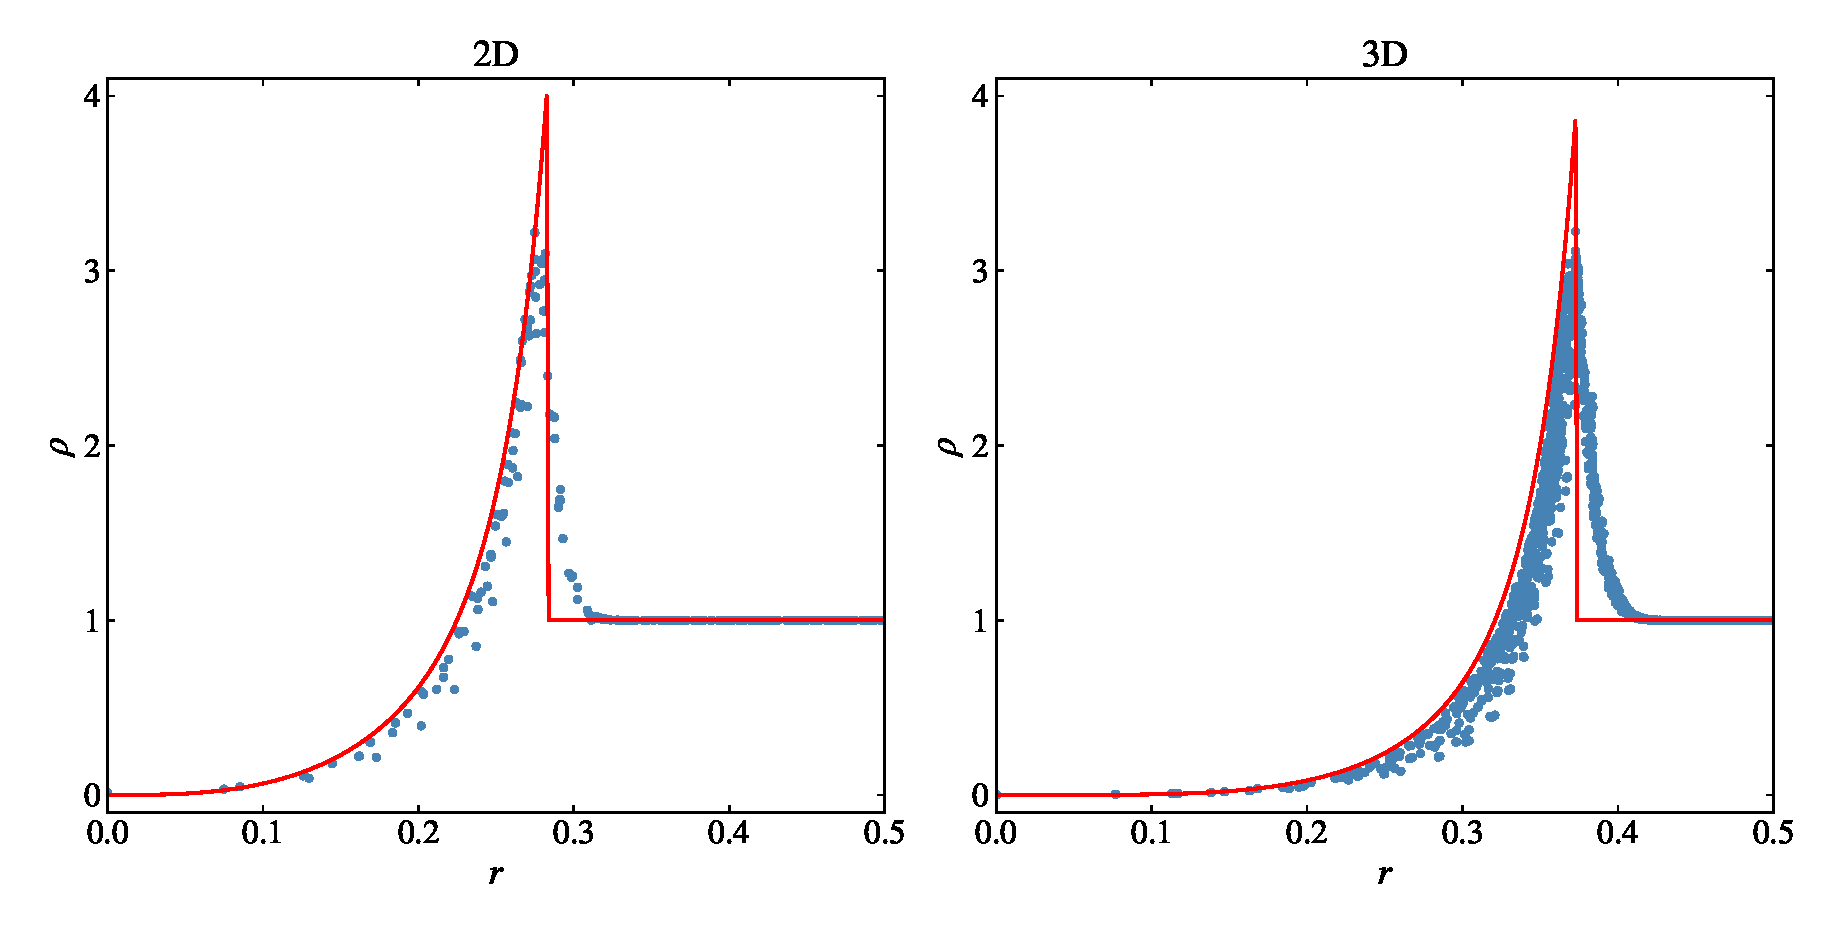
\includegraphics[width=0.9\textwidth]{figures/sedov_compare.eps}
        \caption{Density profile of Sedov-Taylor blast wave problem. Left is the 2D version with an initially
        Cartesian mesh of $45 \times 45$. Right is the 3D version with an initially Cartesian mesh of 
        $45 \times 45 \times 45$. Light blue points are the density a radius $r$ from the center of the explosion
        while the red line is the exact solution.}
        \label{fig.sedov}
    \end{center}
\end{figure}
Figure \ref{fig.sedov} shows the cell density as a function of radial distance from the center of the
explosion. It is noted that shock is well resolved by the cells as the mesh has deformed in such a way
that the shock front contains a large amount of cells which is evident in
Figure \ref{fig.sedov_panel}.
\begin{figure}
    \begin{center}
        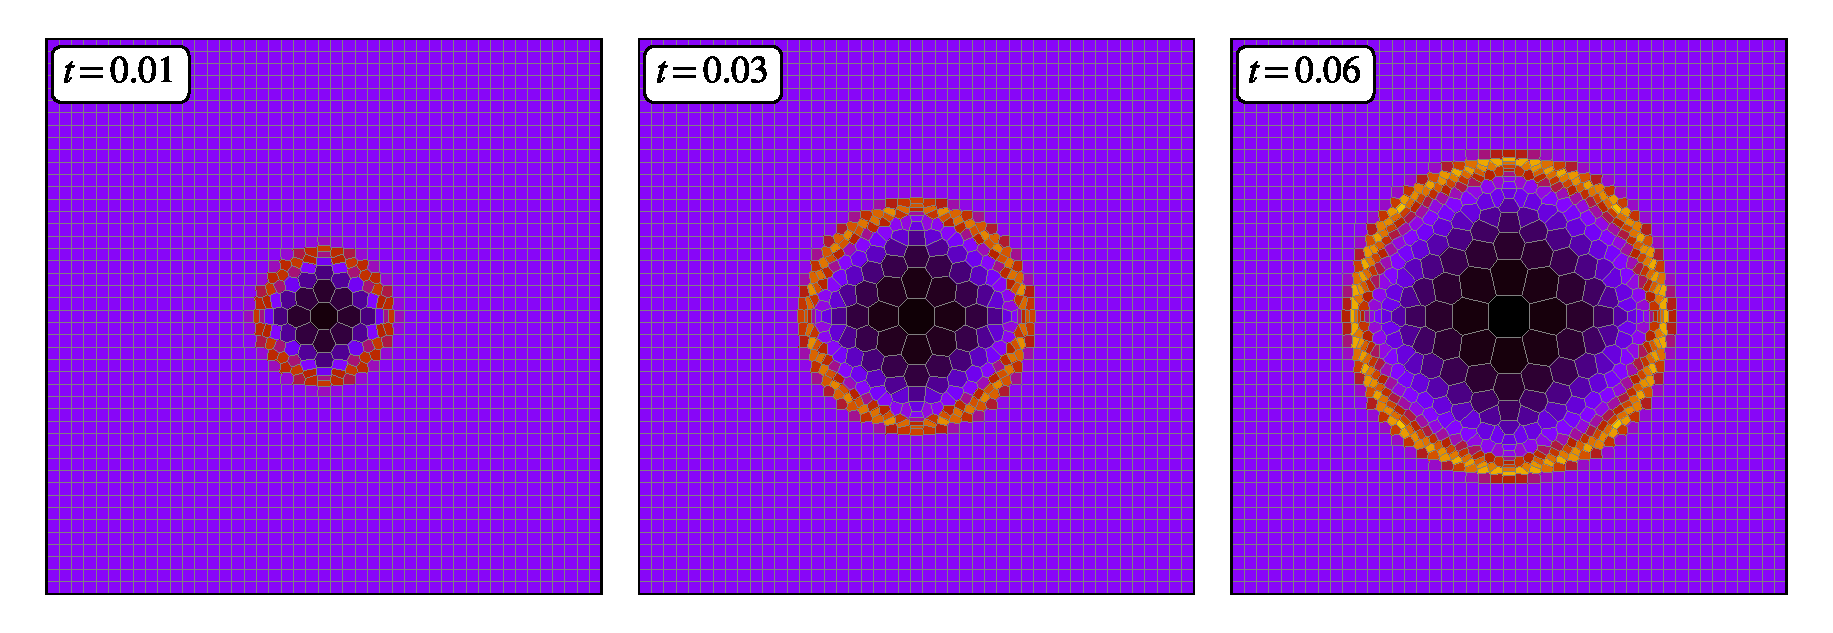
\includegraphics[width=0.9\textwidth]{figures/sedov_panel.eps}
        \caption{Density profile of Sedov-Taylor blast wave problem. Left is the 2D version with an initially
        Cartesian mesh of $45 \times 45$. Right is the 3D version with an initially Cartesian mesh of 
        $45 \times 45 \times 45$. Light blue points are the density a radius $r$ from the center of the explosion
        while the red line is the exact solution.}
        \label{fig.sedov_panel}
    \end{center}
\end{figure}
The center cell, where the energy is deposited, remains stationary while the
cells around it move radially outward. The cells exterior to the shock remain
stationary until they are swept and compressed by the shock.

\subsubsection{Kelvin Helmholtz}

\subsection{Gravity Tests}
\subsubsection{Rayleigh Taylor}
\subsubsection{Two body}
\subsubsection{Evrard Collapse}

\subsection{Chemistry Tests}
\subsubsection{Uniform Cooling}
